%\section{Motivation}
\begin{frame}{Motivation}
	\begin{minipage}{\textwidth}
		\centering		
		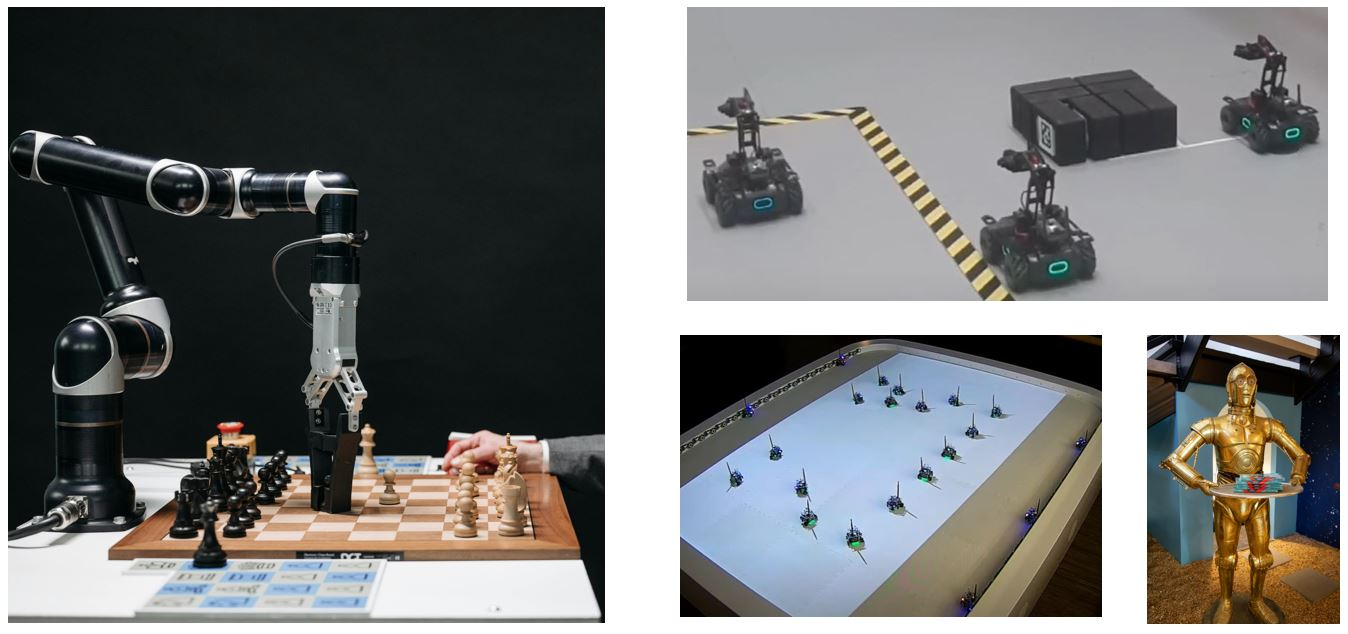
\includegraphics[width=0.85\linewidth]{motivationsCombined}
	\end{minipage}%
	\seprule
	Modern robots are required to do complex tasks and possibly multiple at the same time.
\end{frame}

\begin{frame}
	\begin{itemize}
		\item{Let's use RL to learn several control tasks for a robotic system to execute.}
			\begin{itemize}
				\item{ RL lets us generalize to possibly complex control tasks.}
			\end{itemize}
		\item{Let's combine and execute each of these tasks together.}
			\begin{itemize}
				\item{Preferably in a way that lets us swap out tasks and/or reorder priorities.}
			\end{itemize}
		\item{ { \color{red} How do we know that tasks will not interfere with each other? } }
	\end{itemize}
\end{frame}

\begin{frame}{Assumptions}
	\begin{itemize}
		\item{Assume that our robotic system is control-affine:
	\begin{align*}
		\dot{x} &= f(x) + g(x)u, \,\, x \in \mathbb{R}^n, \,\, u \in \mathbb{R}^p
	\end{align*}}
		\item{Assume that each RL task we learn is encoded with a ``cost-to-go''/value function of the form:
	\begin{align*}
		J_i (x) &\approx \min_{u(\cdot)} \int_t^{\infty} { \color{gray} e^{- \beta \tau} } \left( q_i(x(\tau))) + {\lVert u(\tau) \rVert}^2 \right) d \tau && \text{$q_i$ is P.S.D}
	\end{align*}}
	\end{itemize}
\end{frame}

\section{Key Related Works}

\begin{frame}{Related Work - Combining Learned Tasks Using a Min-Norm Controller}
	\begin{itemize}
		\item{Treat learned value functions as Control Lyapunov Functions}
		\item{Make progress on each task using constrained optimization problem}
	\end{itemize}
	\begin{align*}
		\min_{u \in \mathcal{U}, \delta \in \mathbb{R}^N} \quad & { \lVert u \rVert }^2 \, { \color{gray} + \, \kappa { \lVert \delta \rVert }^2 } \\
		\textrm{s.t.} \quad & L_f {J}_1 (x) + L_g {J}_1 (x) u \le - \sigma_1(x) \, {\color{gray} + \, \delta_1 } \\
                \quad & \vdots \\
		\quad & L_f {J}_N (x) + L_g {J}_N (x) u \le - \sigma_N(x) \, {\color{gray} + \, \delta_N } \\
		\quad & { \color{gray} K \delta \ge 0 }
	\end{align*}
        Note that: $L_f {J}_i(x) = \frac{\partial {J}_i}{\partial x} f(x), \, L_g {J}_i(x) = \frac{\partial {J}_i}{\partial x} g(x)$.\\
	\seprule
	\footnotesize{[1] G. Notomista, “A Constrained-Optimization Approach to the Execution of Prioritized Stacks of Learned Multi-robot Tasks,” in Distributed Autonomous Robotic Systems, 2024, pp. 479–493}
\end{frame}

\begin{frame}{Related Work - Value Iteration for Continuous Action Spaces}
	Assume continuous, control-affine dynamics and cost function as mentioned previously.
	\begin{align*}
		\dot{x} &= f(x) + g(x)u, \,\, x \in \mathbb{R}^n, \,\, u \in \mathbb{R}^p \\
		J_i (x) &\approx \min_{u(\cdot)} \int_t^{\infty} q_i(x(\tau))) + {\lVert u(\tau) \rVert}^2 d \tau
	\end{align*}
	Use expression from solved HJB equation as ``optimal input'' at each iteration.
	\begin{align*}
		u^{\star} &= - \frac{1}{2} ( L_g {J}_i (x) )^{\top} = - \frac{1}{2} g(x)^{\top} \left( \frac{\partial {J}_i}{\partial x} \right)^{\top}
	\end{align*}
	\seprule
	\footnotesize{[2] M. Lutter, S. Mannor, J. Peters, D. Fox, and A. Garg, “Value Iteration in Continuous Actions, States and Time,” in Proceedings of the 38th International Conference on Machine Learning, Jul. 2021, vol. 139, pp. 7224–7234.}
\end{frame}

\begin{frame}{Related Work - Independence and Orthogonality for Robotic Control Tasks}
	\begin{itemize}
		\item{Work in [3] defines notions of independence and orthogonality between Jacobian-based tasks to analyze how multi-joint robot arms can achieve multiple tasks at the same time.}
		\item{Work in [4] define these notions for Extended Set-Based Tasks.}
	\end{itemize}

	\seprule
	\footnotesize{[3] Gianluca Antonelli. 2009. Stability Analysis for Prioritized Closed-Loop Inverse Kinematic Algorithms for Redundant Robotic Systems. IEEE Transactions on Robotics 25, 5 (2009), 985–994}\\
	\footnotesize{[4] Gennaro Notomista, Mario Selvaggio, María Santos, Siddharth Mayya, Francesca Pagano, Vincenzo Lippiello, and Cristian Secchi. 2023. Beyond Jacobian-based tasks: Extended set-based tasks for multi-task execution and prioritization. (2023).}

\end{frame}

\begin{frame}{How do we know that tasks are compatible with each other?}
	\begin{align*}
		\min_{u \in \mathcal{U}, \delta \in \mathbb{R}^N} \quad & { \lVert u \rVert }^2 \\
		\textrm{s.t.} \quad & L_f {J}_1 (x) + { \color{red} L_g {J}_1 (x) } u \le - \sigma_1(x) \\
                \quad & \vdots \\
		\quad & L_f {J}_N (x) + { \color{red} L_g {J}_N (x) } u \le - \sigma_N(x) \\
	\end{align*}
	\centering
	We do not.
\end{frame}

\begin{frame}{Sometimes they are compatible}
	\begin{align*}
		{J}_1 &\rightarrow \textrm{Learn to avoid circular region} \\
		{J}_2 &\rightarrow \textrm{Learn to go to some point}
	\end{align*}
	\begin{minipage}{\textwidth}
		\centering		
		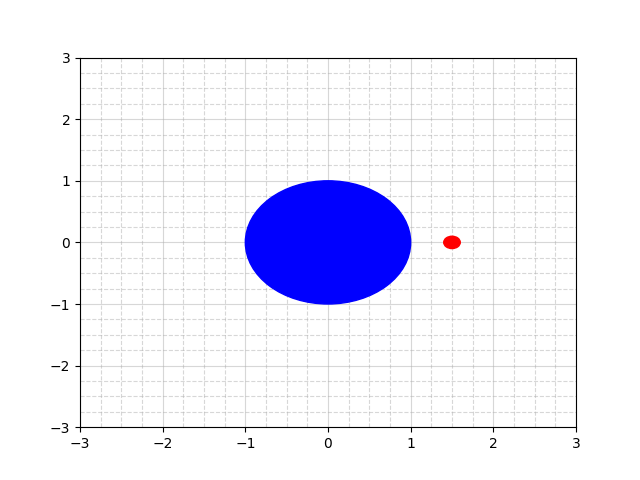
\includegraphics[width=0.5\linewidth]{a1g1}
	\end{minipage}%
\end{frame}

\begin{frame}{Sometimes they are compatible}
	\begin{align*}
		{J}_1 &\rightarrow \textrm{Learn to avoid circular region} \\
		{J}_2 &\rightarrow \textrm{Learn to go to some point}
	\end{align*}
	\begin{minipage}{\textwidth}
		\centering		
		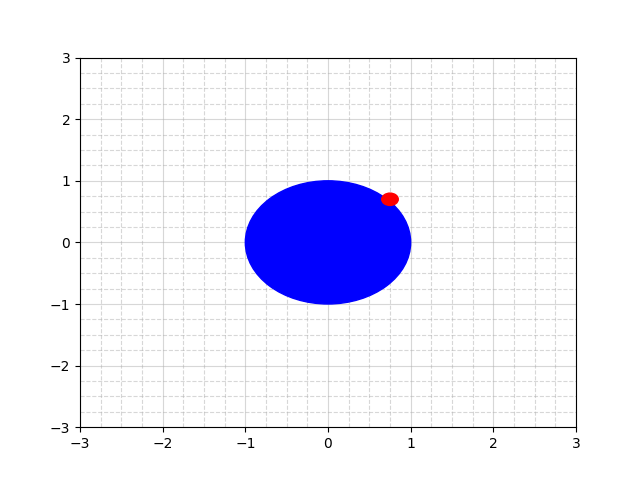
\includegraphics[width=0.5\linewidth]{a1g2}
	\end{minipage}%
\end{frame}


\begin{frame}{Sometimes they are compatible}
	\begin{align*}
		{J}_1 &\rightarrow \textrm{Learn to avoid circular region} \\
		{J}_2 &\rightarrow \textrm{Learn to go to some point}
	\end{align*}
	\begin{minipage}{\textwidth}
		\centering		
		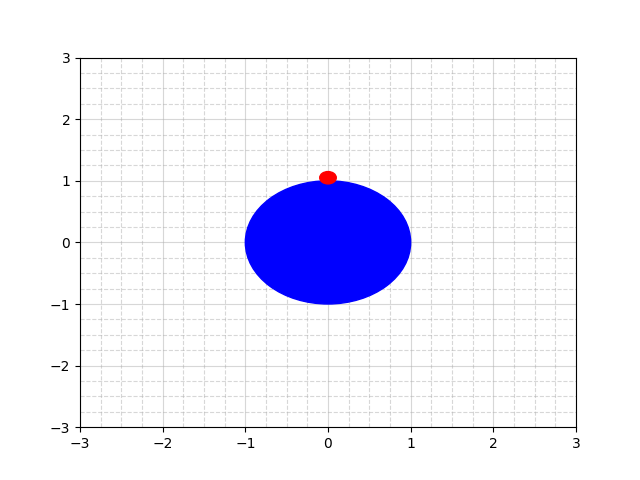
\includegraphics[width=0.5\linewidth]{a1g3}
	\end{minipage}%
\end{frame}

\begin{frame}{Sometimes they are compatible}
	\begin{align*}
		{J}_1 &\rightarrow \textrm{Learn to avoid circular region} \\
		{J}_2 &\rightarrow \textrm{Learn to go to some point}
	\end{align*}
	\begin{minipage}{\textwidth}
		\centering		
		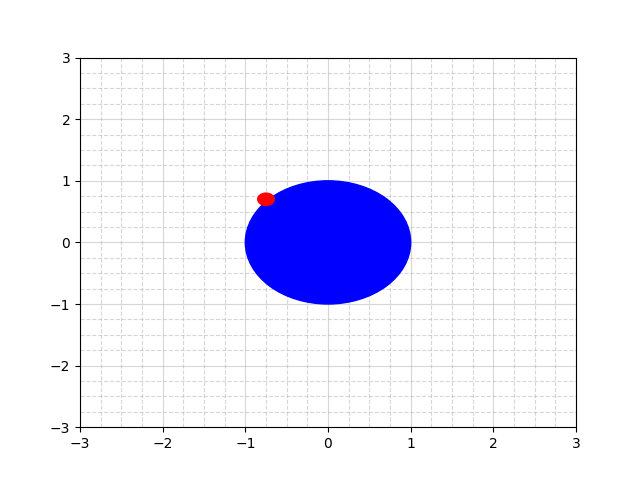
\includegraphics[width=0.5\linewidth]{a1g4}
	\end{minipage}%
\end{frame}

\begin{frame}{Sometimes they are compatible}
	\begin{align*}
		{J}_1 &\rightarrow \textrm{Learn to avoid circular region} \\
		{J}_2 &\rightarrow \textrm{Learn to go to some point}
	\end{align*}
	\begin{minipage}{\textwidth}
		\centering		
		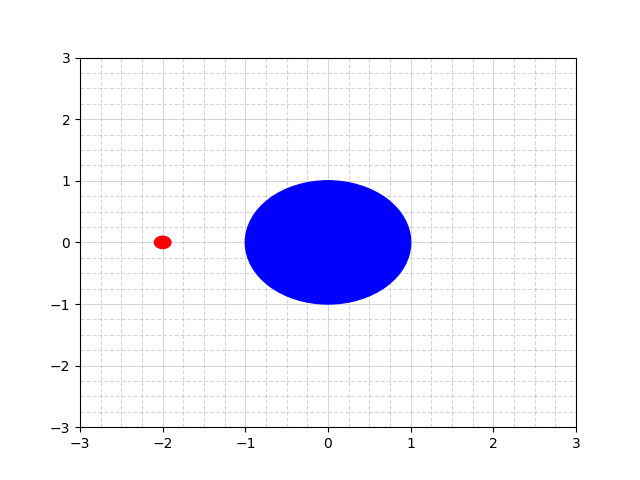
\includegraphics[width=0.5\linewidth]{a1g5}
	\end{minipage}%
\end{frame}


\begin{frame}{Sometimes they are compatible}
	\begin{align*}
		{J}_1 &\rightarrow \textrm{Learn to form a triangle} \\
		{J}_2 &\rightarrow \textrm{Learn to send one robot to a point}
	\end{align*}
	\begin{minipage}{\textwidth}
		\centering		
		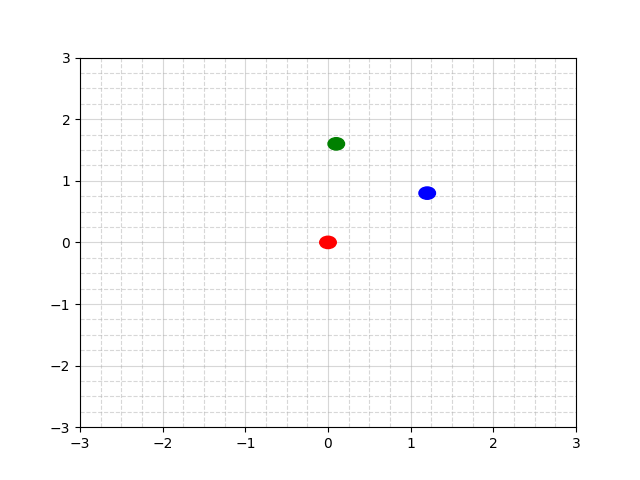
\includegraphics[width=0.5\linewidth]{triangleExample}
	\end{minipage}%
\end{frame}

\begin{frame}{Sometimes they are NOT compatible}
	\begin{align*}
		{J}_1 &\rightarrow \textrm{Learn to avoid square-shaped region} \\
		{J}_2 &\rightarrow \textrm{Learn to go to a point}
	\end{align*}
	\begin{minipage}{\textwidth}
		\centering		
		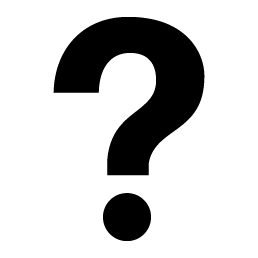
\includegraphics[width=0.3\linewidth]{questionMark}
	\end{minipage}%
\end{frame}

\begin{frame}{Sometimes they are NOT compatible}
	\begin{minipage}{\textwidth}
		\centering		
		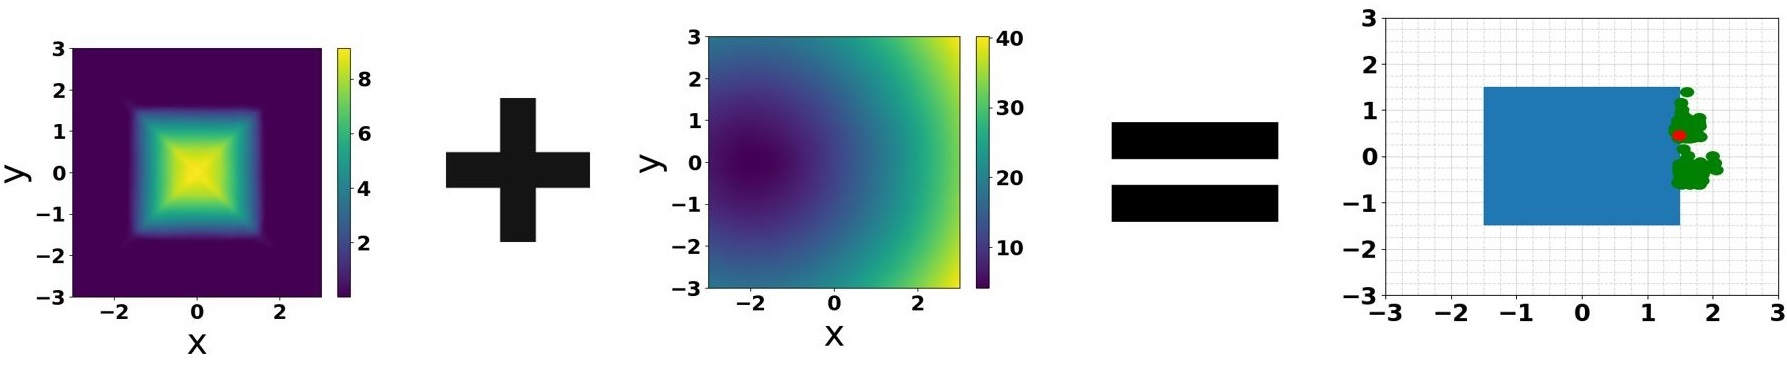
\includegraphics[width=1.\linewidth]{diagramMath}
	\end{minipage}%
	\seprule
	\begin{itemize}
		\item{The above are heat maps of the two value functions.}
		\item{Combining them results in the trajectory on the right.}
	\end{itemize}
\end{frame}

\begin{frame}{Definitions of Independence and Orthogonality}
	\begin{align*}
		\min_{u \in \mathcal{U}, \delta \in \mathbb{R}^N} \quad & { \lVert u \rVert }^2 \\
		\textrm{s.t.} \quad & L_f {J}_1 (x) + { \color{red} L_g {J}_1 (x) } u \le - \sigma_1(x) \\
                \quad & \vdots \\
		\quad & L_f {J}_N (x) + { \color{red} L_g {J}_N (x) } u \le - \sigma_N(x) \\
	\end{align*}
\end{frame}

\begin{frame}{Definitions of \textit{Independence} and \textit{Orthogonality}}
	\centering
	\begin{align*}
		{J}_1, \ldots {J}_N \,\,\, \textrm{are \textit{independent} at $x \in \mathcal{X}$} &\Leftrightarrow L_g {J}_1 (x)^{\top}, \ldots, L_g {J}_N (x)^{\top} \,\,\, \textrm{are linearly independent}\\
		\\
		{J}_1, \ldots {J}_N \,\,\, \textrm{are \textit{orthogonal} at $x \in \mathcal{X}$} &\Leftrightarrow \langle L_g {J}_i (x)^{\top}, L_g {J}_j (x)^{\top} \rangle = 0 \,\,\, \forall \,\, i, j \in \{1,\ldots,N \}
	\end{align*}
\end{frame}

\begin{frame}{Introducing ``Interference'' Input Cost}
	\begin{align*}
		{J}_{N + 1} \approx \min_{u(\cdot)} \int_t^{\infty} { \color{gray}  e^{- \beta \tau } } \left( q_{N + 1}(x) + { \lVert u \rVert }^2 + { \color{red} \sum_{i = 1}^N ( L_g {J}_i (x) u)^2 \lambda_i } \right) d \tau
        \end{align*}
	\seprule
	In Proposition 2, we show that by picking large enough values of $\lambda_i$ and successfully fitting the cost functional, we can make the new task, $J_{N + 1}$, independent to previously trained tasks $J_1, \ldots, J_N$. 
\end{frame}

\begin{frame}{Variant of Value Iteration in Continuous Action Space}
	Can extend previous work in [2] to approximate this new cost functional.
	\begin{align*}
                {J}_{N + 1} \approx \min_{u(\cdot)} \int_t^{\infty} e^{- \beta \tau } \left( q_{N + 1}(x) + { \lVert u \rVert }^2 + { \color{red} \sum_{i = 1}^N ( L_g {J}_i (x) u)^2 \lambda_i } \right) d \tau
	\end{align*}
	At each iteration, use the following input to to estimate the next iteration of the value function.
	\begin{align*}
                u^{\star} &= - \frac{1}{2} {R(x)}^{-1} ( L_g {J}_{N + 1} (x) )^{\top} \\ 
                R(x) &= I + \sum_{i = 1}^N ( L_g {J}_i (x) )^{\top} L_g {J}_i (x)
	\end{align*}
	\seprule
	\footnotesize{[2] M. Lutter, S. Mannor, J. Peters, D. Fox, and A. Garg, “Value Iteration in Continuous Actions, States and Time,” in Proceedings of the 38th International Conference on Machine Learning, Jul. 2021, vol. 139, pp. 7224–7234.}
\end{frame}

\begin{frame}{Relating Orthogonality to the Optimal Input}
Proposition 3:\\
Assume that ${J}_1, \ldots, {J}_N$ are independent at $x \in \mathcal{X}$.\\
If we train a new cost-to-go function, ${J}_{N + 1}$ to be independent to ${J}_1, \ldots, {J}_N$,\\
${J}_{N + 1}$ is orthogonal to each of ${J}_1, \ldots, {J}_N$ at $x \in \mathcal{X}$.\\ 
$\Leftrightarrow$\\ 
the optimal input is $- \frac{1}{2} L_g {J}_{N + 1} (x)^{\top}$.
\end{frame}

\begin{frame}{Now they ARE compatible.}
	\begin{minipage}{\textwidth}
		\centering		
		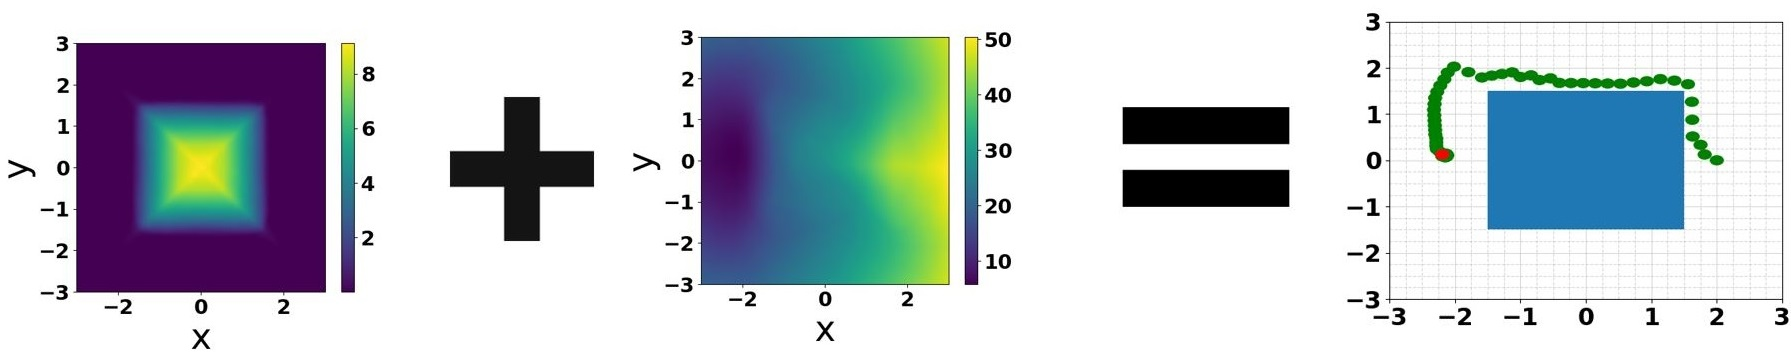
\includegraphics[width=1.\linewidth]{diagramMath2}
	\end{minipage}%
	\seprule
	\begin{itemize}
		\item{The above are heat maps of the two value functions.}
		\item{Combining them results in the trajectory on the right.}
	\end{itemize}
\end{frame}

\begin{frame}{We tried our idea on other scenarios.}
	\begin{minipage}{\textwidth}
		\centering		
		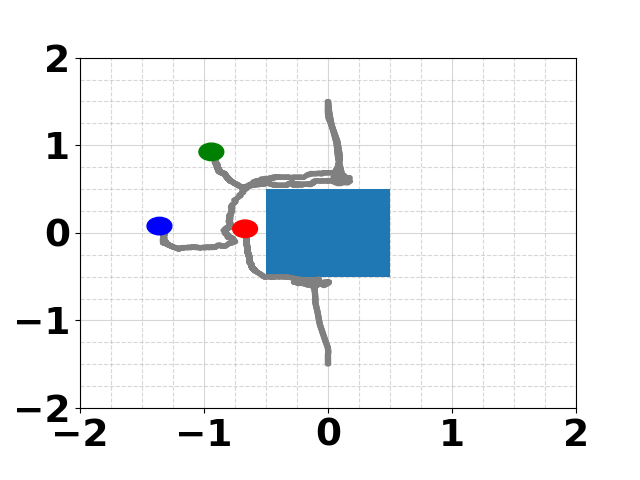
\includegraphics[width=0.4\linewidth]{multRobotSim1}
		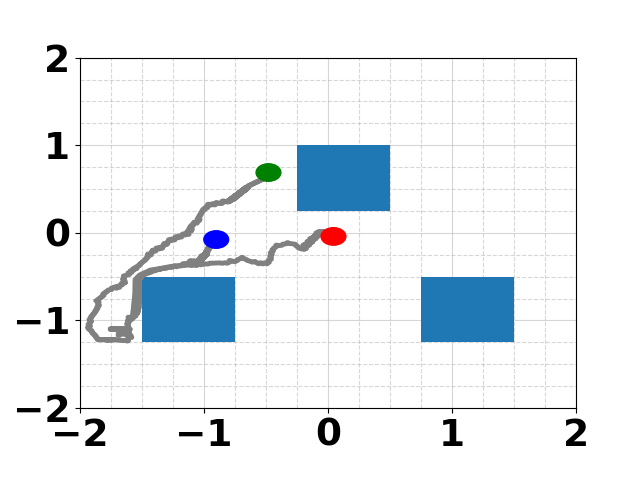
\includegraphics[width=0.4\linewidth]{multRobotSim2}
		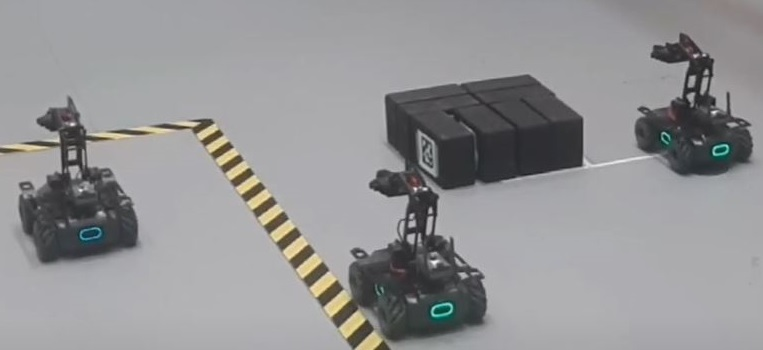
\includegraphics[width=0.4\linewidth]{multiRobotRoboHub}
	\end{minipage}%
\end{frame}

\begin{frame}{Summary of Contributions}
	\begin{itemize}
		\item{Defined notions of independence and orthogonality for learned value functions}
		\item{Introduced ``interference'' for encouraging newly trained value functions to be independent to previous ones}
		\item{Introduced variant of value iteration for continuous input/action space that can fit cost functionals with this new ``interference'' cost}
		\item{Tested our idea in a few different scenarios involving controlling a team of mobile robots}
	\end{itemize}
\end{frame}

\end{document}

